%%%%%%%%%%%%%%%%  DISCUSSION  %%%%%%%%%%%%%%%%%%%%%
\chapter{Discussion} \thispagestyle{chapterpage}
\label{chapter:discussion}

\section{Convergence tests}
\label{section:discussion_convergence_tests}
We restate the viscosity residual from Equation (\ref{eq:residual_two_phase_transport}) with simplified notation:
\begin{equation} \label{eq:residual_two_phase_transport_simple}
R(S^{n+1};q_i,q_o,M,\tau) = S^{n+1} - S^{n} + \tau \left(q_o f_w(S^{n+1}) + q_i\right) = 0
\end{equation}
Here $\tau$ is defined by
\begin{equation*}
\tau = \frac{\Delta t}{m(V) \phi_V}.
\end{equation*}
The dynamics of the fluid flow is embedded in the last term of the Equation (\ref{eq:residual_two_phase_transport_simple}), i.e. $\tau \left(q_o f_w(S^{n+1}) + q_i\right)$. We call this the \emph{flow term} of the transport equation. The observations from the convergence tests in Section \ref{section:numerical_results_convergence_tests} indicates that the cell saturation from the previous transport step can be a determining factor for the root placement. We now seek to investigate under which circumstances this is the case. Since the saturation $S^n \in [0,1]$, we have a well defined range for the size of the two first terms in Equation (\ref{eq:residual_two_phase_transport_simple}). This implies that the old cell saturation $S^n$ is significant when $\tau \left(q_o f_w(S^{n+1}) + q_i\right) \approx 1$, in the sense that the size of the flow term is of the same order of magnitude as the number $1$. Of course, $S^{n+1} = S^n$ when $\tau \left(q_o f_w(S^{n+1}) + q_i\right) = 0$. Likewise, when the flow term is much larger than $1$, the solution $S^{n+1}$ is completely dominated by the fractional flow function $f_w$ and the flux terms $q_i$ and $q_o$. These facts explains the observations made based on the convergence plots in Section \ref{section:numerical_results_convergence_tests}. As stated, the size of the flow term in Equation (\ref{eq:residual_two_phase_transport_simple}) is determined by the incoming and outgoing fluxes, and the factor $\tau$. The fluxes measure the magnitude of flow in and out of the current cell, while $\tau$ gives the time-volume scale of the flow. That is, $\tau$ measures the number of seconds the fluxes $q_i$ and $q_o$ are allowed to move across the cell boundaries per volume unit of the cell. In practice this leads to small cells being drained faster than larger cells, and a larger flow in each iteration for large time steps.

It is of interest to know \emph{a priori} under which circumstances the old saturation value is a good starting guess for the root finders. We investigate this by assuming $q_o, q_i \gg 1$. Then, dividing Equation (\ref{eq:residual_two_phase_transport_simple}) by $q_o$ we obtain
\begin{equation*}
\frac{S^{n+1}}{q_o} - \frac{S^n}{q_o} + \tau f_w(S^{n+1}) + \tau \frac{q_i}{q_o} = 0.
\end{equation*}
Since $q_0 \gg 1$, $\frac{S^{n+1}}{q_o} \ll 0$ and $\frac{S^n}{q_o} \ll 1$. Having assumed quadratic relative permeabilities $k_{rl}$ the shape of the fractional flow function $f_w(S;M)$ is as shown in Figure \ref{fig:fractional_flow_wrt_viscosity_ratio} for varying viscosity ratios $M$. 
\begin{figure}[ht]
\tikzsetnextfilename{fractional_flow_wrt_viscosity_ratio}
\centering
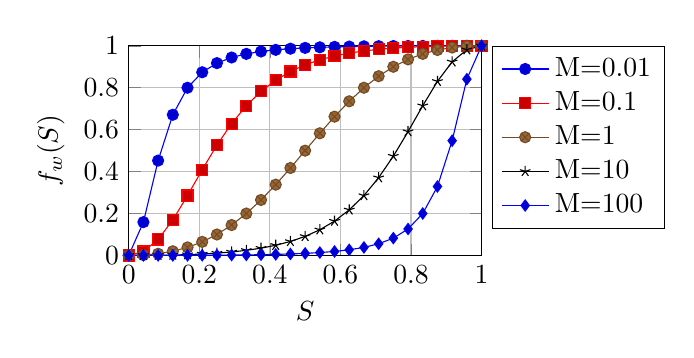
\begin{tikzpicture}
\begin{axis}[
	width=0.5\textwidth,
	height=0.35\textwidth,
	xlabel={$S$},
	ylabel={$f_w(S)$},
	xmin = 0,
	xmax = 1,
	ymin = 0,
	ymax = 1,
	domain = 0:1,
	%samples = 100,
	grid = major,
	legend style={
		cells={anchor=west},
		legend pos=outer north east,
	}
	]
	\addplot {x^2/(x^2+0.01*(1-x)^2)};
	\addplot {x^2/(x^2+0.1*(1-x)^2)};
	\addplot {x^2/(x^2+1*(1-x)^2)};
	\addplot {x^2/(x^2+10*(1-x)^2)};
	\addplot {x^2/(x^2+100*(1-x)^2)};
	\legend{M=0.01,M=0.1,M=1,M=10,M=100}
\end{axis}
\end{tikzpicture}
\caption{The fractional water flow function $f_w$, Equation (\ref{eq:fractional_flow_function}), with quadratic $k_{rl}$ and viscosity ratio $M$, Equation (\ref{eq:viscosity_ratio}).}%
\label{fig:fractional_flow_wrt_viscosity_ratio}%
\end{figure}%
We observe that $M > 1$  gives $f_w$-values closer to unity on the left hand side, while $M < 1$ brings the left hand side values of $f_w$ close to zero, leaving a smaller region close to unity for $S > \frac{1}{2}$. Still, $f_w(S = 0;M) = 0$ for all $M > 0$. Thus, if 
\begin{equation*}
\lvert \tau \frac{q_i}{q_o} \rvert \approx  1,
\end{equation*} 
and since $\tau f_w \ll 1$ for ``small enough'' $S^{n+1}$, the old cell saturation $S^n$ is significant for determining the root. On the other hand, if 
\begin{equation*}
\lvert \tau \frac{q_i}{q_o} \rvert \gg 1,
\end{equation*}
we expect the root to be invariant under $S^n$ since this term will dominate the $S^n$ influence even for small $\tau f_w$.

